\documentclass[11pt]{article}
\usepackage{aas_macros}
\usepackage{hyperref}
\usepackage[hmargin=1.5cm, vmargin=0.55cm]{geometry}
\usepackage{amsmath}
\usepackage{caption}
\usepackage{mathtools}
\usepackage{fancyhdr}
\usepackage{float}%Places the float at precisely the location in the LaTeX code...i.e, [H]
\usepackage{wrapfig}
\usepackage{graphicx}%includegraphics
%converts eps to pdf
%\usepackage{subcaption} %need to find subcaption.sty for this to work!
%\usepackage{epstopdf}
\DeclareGraphicsExtensions{.pdf,.png,.jpg,.eps}
\renewcommand{\vec}[1]{\mathbf{#1}}
\usepackage[round]{natbib}  %use the "Natbib" style for the references in the Bibliography
%\usepackage{aastex}%defines journal abbreviations in bib file



\title{Probation Report}
\author{Jamie Ryan \\ 
Mullard Space Science Laboratory \\
University College London \\
Surrey, RH13 6NL, UK\\
\href{mailto:jamie.ryan.14@ucl.ac.uk}{jamie.ryan.14@ucl.ac.uk}
\date{}}
\begin{document}
\maketitle


\section{Introduction}


\subsection{Solar Magnetohydrodynamics}\label{MHD}
Most structures observed in the solar atmosphere are a direct result of interplay between plasma and the Sun's dynamic magnetic field. Understanding the relationship between a magnetic field and a plasma is important for describing many observed phenomena. Magnetohydrodynamics (MHD) is a method to determine the continuous macroscopic behaviour of plasma in a magnetic field, thus individual particles are not considered \citep{1982soma.book.....P}. A plasma can be treated as a continuous material if distances between particles are much larger than the mean-free path, or larger than the ion gyro-radius. Where $T$ is plasma temperature, $\lambda_{MFP}$ is mean-free path and $n$ is number of particles in the plasma, equation \ref{meanfreepath} describes the mean-free path. 

\begin{equation}\label{meanfreepath}
\lambda_{MFP}\approx300(\frac{T}{10^{6}K})^{2}(\frac{n}{10^{17}m^{-3}})^{-1}m
\end{equation}

Equation \ref{iongyroradius} is the relationship between particle mass $m$, velocity perpendicular to the magnetic field $v_{\bot}$, charge $q$ and magnetic field strength $B$  which governs the circular motion of a charged particle around a uniform magnetic field or the ion gyro radius. 

\begin{equation}\label{iongyroradius}
r_{g}=\frac{mv_{\bot}}{|q|B}
\end{equation}

In the context of the Sun, and the importance of magnetic fields for processes such as solar flares, MHD builds on the following physical assumptions; a magnetic field can manipulate a plasma by exerting a force on it. Leading to the formation of structure or movement via acceleration; a magnetic field can store the energy required for later release as a solar flare; material wrapped in a magnetic field is thermally protected from it's surroundings; a magnetic field can act as a funnel for plasma and fast particles; and finally, a magnetic field can drive instabilities and support waves \citep{2003dysu.book.....D}.

\subsubsection{MHD Equations}\label{MHDeqns}
Magnetic fields are made up of discreet bundles of magnetic flux known as \emph{flux tubes}. A magnetic flux tube can be thought of as cylindrical in geometry and containing magnetic field lines parallel in orientation to the length of the cylinder. The cross-sectional radius of the tube and magnetic field strength are both variant, magnetic flux contained within the tube however, is constant. Where $\vec{B}$ is magnetic field vector and $\vec{dS}$ is a cross-sectional surface element of the tube, flux $F$ follows the relationship.

\begin{equation}\label{fluxtube}       
F = \int_{S} \vec{B}.\vec{dS}
\end{equation}


The basics of MHD are a built from a combination of Maxwell's electromagnetic equations, material equations, Ohm's law and the fluid dynamics relations. Maxwell's equations and Ohm's law describe electromagnetism in terms of magnetic field $\vec{H}$, magnetic induction $\vec{B}$, magnetic permeability of free space $\mu$, electric field $\vec{E}$, electric displacement $\vec{D}$, electrical permittivity of free space $\epsilon$, charge density $\rho_{c}$ and electric current density $\vec{j}$ 


\begin{equation}\label{max1:ampere}
\nabla\times\vec{H}=\vec{j}+\frac{\partial \vec{D}}{\partial t}
\end{equation}


\begin{equation}\label{max2:faraday}
\nabla\times\vec{E}=-\frac{\partial \vec{B}}{\partial t}
\end{equation}


\begin{equation}\label{max3:gauss}
\nabla\cdot\vec{D}=\rho_{c}
\end{equation}


\begin{equation}\label{max4:nomonopole}
\nabla\cdot\vec{B}=0
\end{equation}

with Ohm's law as,

\begin{equation}\label{ohmslaw}
\vec{E}=\frac{\vec{j}}{\sigma}
\end{equation}

where $\sigma$ is electrical conductivity. The fluid dynamics relations are written in terms of density $\rho$, velocity $\vec{v}$, time $t$, pressure $p$, gas constant $\Re$ and temperature $T$. 
%$\frac{d}{dt}=\frac{\partial}{\partial t}+ \vec{v}\cdot\nabla$, sometimes reffered to as the material derivative, is a way of stating the rate of change with respect to time of the  

\begin{equation}\label{motion}
\rho\frac{d\vec{v}}{dt}=-\nabla p
\end{equation}
 
\begin{equation}\label{masscontinuity}
\frac{d\rho}{dt}+\rho\nabla\cdot\vec{v}=0
\end{equation}

\begin{equation}\label{perfectgaslaw}
p=\Re\rho T
\end{equation}

Equation \ref{motion} is the eqn. of motion describing how the forces are exerted on the fluid are equal to the negative gradient of plasma pressure. Equation \ref{masscontinuity} is the eqn. of mass continuity (mass is conserved), whilst equation \ref{perfectgaslaw} is the perfect gas law relating plasma pressure, density and temperature. The fluid dynamics equations are re-written in terms of MHD by building on the following assumptions: Plasma in a magnetic field experiences the Lorentz force $(\vec{j}\times\vec{B})$, such that a plasma volume element $dV$ carrying a current density $\vec{j}$ per unit volume has the force $\vec{j}dV\times\vec{B}$ exerted on it in a perpendicular direction to the magnetic field. In order to cater for the extra force, equation \ref{motion} has the term $\vec{j}\times\vec{B}$ added to the right hand side.   
Ohm's law states that an electric field in the plasma's frame of reference is proportional to the current, however, the total electric field associated with the movement of plasma is $\vec{E}+\vec{v}\times\vec{B}$ ($\vec{E}$ is the electric field acting on the plasma at rest) therefore, equation \ref{ohmslaw} has the term $\vec{v}\times\vec{B}$ added to it's left hand side.The displacement current term $\frac{\partial \vec{D}}{\partial t}$ in equation \ref{max1:ampere} is neglected due to plasma speeds being much slower than the speed of light.

\subsubsection{Induction Equation}\label{inductioneqn}  
Rewriting equations \ref{max1:ampere}, \ref{max2:faraday} and \ref{ohmslaw} using the assumptions from section \ref{MHDeqns}, with $\nabla\cdot\vec{B} = 0$,

\begin{equation}\label{new1}
\vec{j}=\nabla\times\frac{\vec{B}}{\mu}
\end{equation}

\begin{equation}\label{new2}
\frac{\partial \vec{B}}{\partial t} = - \nabla\times\vec{E}
\end{equation}

\begin{equation}\label{new3}
\vec{E}=-\vec{v}\times\vec{B}+\frac{\vec{j}}{\sigma}
\end{equation}

then substituting \ref{new1} solved for $\vec{j}$ into \ref{new2} we have,

\begin{equation}\label{new4} 
\vec{E}=-\vec{v}\times\vec{B}+\nabla\times\frac{\vec{B}}{\eta} 
\end{equation}

where magnetic diffusivity $=\eta =\frac{1}{\mu\sigma}$.

Substituting \ref{new4}, solved for $\vec{E}$, into \ref{new2},

\begin{equation}\label{new5}
\frac{\partial \vec{B}}{\partial t}=-\nabla\times(-\vec{v}\times\vec{B} + \nabla\times\vec{B}\eta)
                                   =\nabla\times(\vec{v}\times\vec{B})-\nabla\eta\times(\nabla\times\vec{B})
\end{equation}

using the vector identity, $\nabla\times(\nabla\times\vec{A})=\nabla(\nabla\cdot\vec{A})-\nabla^{2}\vec{A}$ the last term in equation \ref{new5} becomes $\nabla(\nabla\cdot\vec{B})-\nabla^{2}\vec{B}$, of which the $\nabla\cdot\vec{B}$ term reduces to zero due to equation \ref{max4:nomonopole}, thus we are left with the induction equation \ref{induction} below. 



\begin{equation}\label{induction}
\frac{\partial \vec{B}}{\partial t}=\nabla\times(\vec{v}\times\vec{B})+\eta\nabla^{2}\vec{B}  
\end{equation}

This equation \ref{induction} can be used to determine $\vec{B}$ if $\vec{v}$ is known. The magnetic Reynolds number,

\begin{equation}\label{reynolds}
R_{m} = \frac{l_{0}v_{0}}{\eta} \sim \frac{\nabla\times(\vec{v}\times\vec{B})}{\eta\nabla^{2}\vec{B}}
\end{equation}

is an approximation of the ratio between the first and second terms on the RHS of the induction equation \ref{induction} if $v_0$ and $l_0$ are typical of the velocity and length-scales over which the system is changing. This ratio can be used to diagnose which part of the induction equation is dominating the MHD of the system. For example if $R_m >> 1$ then the $\nabla\times(\vec{v}\times\vec{B})$ term is large and the second term is negligible, so the induction equation becomes,

\begin{equation}\label{r>>1}
\frac{\partial \vec{B}}{\partial t}=\nabla\times(\vec{v}\times\vec{B}),
\end{equation}

thus induction is dominant and Ohm's law \ref{ohmslaw} becomes $\vec{E} +\vec{v}\times\vec{B}$ meaning the total electric field becomes zero.



If $R_m << 1$ then the $\eta\nabla^{2}\vec{B}$ term is large meaning the induction equation becomes,
\begin{equation}\label{r<<1}
\frac{\partial \vec{B}}{\partial t}=\eta\nabla^{2}\vec{B},
\end{equation}

thus diffusion is dominant so the magnetic field $\vec{B}$ will be varying on a length-scale $L_0$, and so will diffuse with velocity \ref{diffvel}, over the time-scale \ref{difftime}.

\begin{equation}\label{diffvel}
v_d=\frac{L_0}{\tau_d} = \frac{\eta}{L_0}
\end{equation}


\begin{equation}\label{difftime}
\tau_d = \frac{L_{0}^{2}}{\eta}
\end{equation}

%check Foukal pg 125 in the pdf
\citep{2003dysu.book.....D}

%puts .tex file here
%\include{example}
\subsubsection{Plasma Beta}
Another way to write the relationship between $\vec{B}$ and $\vec{v}$ is the equation of motion \ref{motion} modified by the Lorentz force.

\begin{equation}\label{motion1}
\rho\frac{d\vec{v}}{dt}=-\nabla p+\vec{j}\times\vec{B}
\end{equation}

The pressure gradient $-\nabla p$ describes the change from high to low plasma pressure. The Lorentz force, $\vec{j}\times\vec{B}$ acts perpendicularly to the magnetic field, therefore accelerated plasma in a direction parallel to the magnetic field is caused by other forces. If equation \ref{new1} is substituted into the Lorentz force,
\begin{equation}\label{lorentzsub1}
\vec{j}\times\vec{B} = (\nabla\times\frac{\vec{B}}{\mu})\times\vec{B}
\end{equation}

then using the triple vector identity, 
\begin{equation}
\frac{1}2{}\nabla(\vec{B}\cdot\vec{B})=\vec{B}\times(\nabla\times\vec{B})+(\vec{B}\cdot\nabla)\vec{B}
\end{equation}

equation \ref{lorentzsub1} becomes,
\begin{equation}
\vec{j}\times\vec{B} = (\vec{B}\cdot\nabla)\frac{\vec{B}}{\mu}-\nabla(\frac{B^2}{2\mu}) 
\end{equation}

therefore \ref{motion1} becomes:

\begin{equation}\label{maghydstat}
\rho\frac{d\vec{v}}{dt}= -\nabla p + (\vec{B}\cdot\nabla)\frac{\vec{B}}{\mu}-\nabla(\frac{B^2}{2\mu}) 
\end{equation}

Because $-\nabla(\frac{B^2}{2\mu}$ is in the same form as $-\nabla p$ it can be said to be the \emph{magnetic pressure}, providing a force pointing from high to low magnetic pressure as $B^2$ changes with position.A measure of dominance of plasma or magnetic pressure in the motion of plasma is known as the plasma beta, 

\begin{equation}\label{beta}
\beta=\frac{p_{plasma}}{p_mag} = \frac{2p_{0}\mu}{B_{0}^2}
\end{equation}

so if $\beta << 1$ then magnetic pressure is dominant and if $\beta >> 1$ then plasma pressure is dominant.

Another useful relationship to use is pressure scale height, where $g$ is acceleration due to gravity and $T_0$ is uniform temperature, pressure scale height, $H=\frac{P_0}{\rho_{0}g} = \frac{\Re T_{0}}{g}$. When combined with pressure, $p$ for a magneto static plasma with uniform temperature, $p=p_{0}\exp^{\frac{-z}{H}}$, where $z$ is altitude, we have a measure of the height, $H$, over which the pressure of a plasma fall off by a factor of $\exp$. 



\subsection{Solar Atmosphere}\label{ATM}
The solar atmosphere \citep{2003dysu.book.....D, 2004soas.book.....F} is described as having four main components, the corona, transition region, chromosphere and photosphere. The photosphere is the lowest in altitude of the four layers characterised as having an effective temperature $T=5800$K, the photosphere decreases in temperature with radial distance. Due to the assumption that this region emits as a black body the temperature is estimated using Wien's displacement law. Pressure scale height in this part of the atmosphere is $H\sim150$km. The plasma beta in this region is mostly larger than one $\beta >1$ meaning plasma pressure is the dominant force dictating plasma motions, the exception to this exists in sunspots where $\beta<1$ and magnetic pressure is dominant. Dark, lower temperature patches found in active regions of the photosphere, sunspots are regions of intense magnetic field. They are made up of two main parts, the central umbra, surrounded by the slightly less dark penumbra. The umbra hosts magnetic field lines that are tightly packed and pointing radially away from the Sun, whereas the penumbral magnetic field is more horizontal. Other features that are part of the photosphere include granules and super granules (seen only in Doppler images), which are the physical representation of convection currents. Heated plasma rises from below the surface and is seen as the bright central part of the granule, the darker surrounding regions are cooler material sinking back into the interior. The next region of the atmosphere is the chromosphere which is situated above the photosphere. This layer of plasma is a few thousand kilometres (2000-3000km) thick and is optically thin to visible light so is difficult to see against the brightness of the photosphere. The temperature in this layer increases with height and ranges from 4400K at the temperature minimum region to $\sim10^{5}$K at the top, as a result, $\beta$ drops rapidly crossing unity as it does so. The pressure scale height, based on an average isothermal temperature of $2\times10^{4}$ is $H\sim600$km. The dominant emission in this region is H$\alpha$ at $6563\AA$.

\begin{wrapfigure}{R}{0.48\textwidth}
  %\begin{center}
    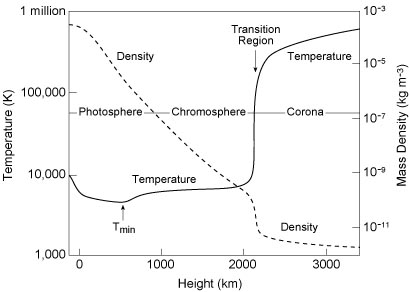
\includegraphics[width=0.45\textwidth]{solar-atm-plot}
  %\end{center}
\caption{The temperature of the solar atmosphere decreases from values near 6,000 degrees Kelvin at the visible photosphere to a minimum value of roughly 4,400 degrees Kelvin about 500 kilometers higher up. The temperature increases with height, slowly at first, then extremely rapidly in the narrow transition region, less than 100 kilometers thick, between the chromosphere and corona, from about $10^{4}$K to about $10^{6}$K. (Courtesy of Eugene Avrett, Smithsonian Astrophysical Observatory.) }\label{solatm}
\end{wrapfigure}

Through the transition region to the corona and the atmosphere starts to heat considerably to $T\sim10^{7}$K. This region is visible in white light due to Thompson scattering of photospheric light by free electrons and dust in the coronal magnetic field. The plasma beta is less than one through the entire corona meaning magnetic forces dominate and the pressure scale height is approximately $100$Mm.  

\subsection{Eruptive Flare Model}\label{EFM}
Solar flares are the manifestation of magnetic energy release in the form of electromagnetic radiation spanning a wide range of wavelengths. These events are the most energetic phenomena associated with the Sun, with some of the larger flares releasing $10^{37}$ erg of energy. Flares are classified by the X-ray flux measured by the Geostationary Operational Environmental Satellite (GOES) see \ref{GOES}.

\begin{table}[h]
%\captionsetup{justification=raggedright,singlelinecheck=false}

\centering
\begin{tabular}{|c|c|}
Classification & Peak Flux Range ($W.m^{-2}$)\\ 
X & $10^{-3}$ - $10^{-4}$\\ 
M & $10^{-4}$ - $10^{-5}$\\ 
C & $10^{-5}$ - $10^{-6}$\\ 
B & $10^{-6}$ - $10^{-7}$\\ 
A & $<10^{-7}$\\  
\end{tabular}
\caption{Shows the GOES classification of solar flares by measure of X-ray flux at $1$ to $8\AA$}\label{GOES}
\end{table}

The exact physical process governing the mechanics of solar flares is not known, however, magnetic reconnection is the currently accepted mechanism. Coronal magnetic loops tethered to sunspots of opposing polarity in the photosphere and sub-photosphere are twisted and stressed by movements of active regions across the solar surface. This shearing of the magnetic field, effectively stores energy as magnetic tension which can be released when opposing field lines meet and reconnect. The process of energy conversion is basically a unstable tensioned magnetic field relaxing back to a more stable configuration. As a result stored magnetic energy is converted to radiation, kinetic and thermal energy\citep{1976SoPh...50...85K}.\\
The standard 2D flare model is the culmination of many papers by many authors,\citep{1964NASSP..50..451C, 1966Natur.211..695S, 1974SoPh...34..323H, 1976SoPh...50...85K}, and is still an ongoing area of research that is not well understood. In an active region, a closed magnetic field harbouring a prominence suddenly opens. As a result, plasma flows from the chromosphere to the corona. Because material in the chromosphere is denser than in the corona, flowing plasma experiences a drop in plasma pressure and an increase in magnetic pressure. This leads to reconnection of the open magnetic field lines, forming new loops at lower altitudes. Reconnection causes excess heating at the peaks of newly connected loops which conducts down toward the chromosphere. Also, particles are accelerated by the new magnetic configuration, flowing to the chromosphere. This injection of thermal energy and accelerated particles heats the chromosphere causing HXR footpoints \citep{1995ApJ...455..347A} and UV ribbons \citep{2009A&A...493..241F}. As a result, some chromospheric material evaporates upward into newly created flare loops, whilst some material propagates downward toward the lower chromosphere, known as condensation. The flare loop cools and the process starts again in the next consecutive loop until the unstable magnetic field has relaxed to a state that is closer to it's stable,  potential state. In eruptive flares, energy is released every time a new reconnection of a neighbouring loop occurs, this said to be the reason that flare ribbons move away from each other as the flare evolves. 

White light flares are said to be rare events only associated with the most energetic of solar flares, they occur when flare energy is transported deep into the dense lower atmosphere causing an enhancement in optical wavelengths. It is thought this happens due to an electron beam transporting energy to the lower atmosphere where it's energy dissipates into the dense chromospheric or photospheric material. The collisional thick target model by \cite{1971SoPh...18..489B} says that almost all of the flare energy is carried by the electron beam, therefore, energy dissipated in the lower atmosphere represents a large portion of the flare energy budget. White light enhancement from the lower atmosphere can be explained by either, Balmer \& Paschen continuum emission from the chromosphere caused by hydrogen recombination or direct photospheric heating \citep{2007ASPC..368..417D}.    


\subsection{Introduction to Local Helioseismology}\label{HSM}
Helioseismology is a tool for probing the interior of the Sun. Most techniques in this field of analysis rely on observations of gravity and acoustic waves on the photosphere that are the result of interior excitation. Studying the frequency and modes of these oscillations has revealed much about the internal structure of the Sun. Local helioseismology then is a collection of techniques developed for global helioseismology have been modified for use in studying local regions in higher spatial resolution. The following section provides a very basic introduction to some of these techniques. 

\subsubsection{Helioseismic Holography}\label{helioholog}
Originally the idea of analysing Doppler images of the solar surface in order to observe acoustic sources was put forward by \cite{1975CRASB.281...93R}. Helioseismic holography was developed further in concept by Lindsey and Braun \citep{1990SoPh..126..101L, 1992ApJ...392..739B, 1997ApJ...485..895L} in an effort to to image the solar interior and far-side of the Sun. This technique involves using a Doppler image as a representation of the wave-field at a location on the solar surface as a reference point to be able to estimate that wave-field a location in the solar interior at a time preceding or proceeding the image. This is achieved by calculating the ingression or egression of the wave-field by assuming that it's evolution is a, convergence to, or divergence from, the point of origin of that wave-field.  

\subsubsection{Ring Diagram}\label{ring}
\cite{1988ApJ...333..996H} was the first to apply this technique, which is taken from global helioseismology. Frequency images of rings made up of peaks representing two different wavenumber directions can be used to probe the physical conditions of the solar interior. The shape and location of the rings determine local physics. Ring location is dictated by the propagation speed of waves. The shape of the rings are dependant on the state of the thermodynamics below the photosphere.  

\subsubsection{Hankel Analysis}\label{hankel}
This method was originally used to study the inward and outward movements of p-mode waves ($5$ minute oscillations caused by convective motions of the photosphere) about sunspots by \cite{1987ApJ...319L..27B}. The idea is based on splitting a signal into spherical components of azimuthal order, spherical harmonic degree and frequency, then calculating a numerical approximation of the energy of wave components entering and leaving a system. Using this technique, \cite{1987ApJ...319L..27B} was able to measure decrease in power between waves entering and leaving a sunspot.    


\subsubsection{Time-Distance}\label{TD}
The paper by \cite{1993Natur.362..430D} explains how to extract time-distance (TD) information from observations of intensity fluctuations on the solar surface. This technique uses travel times of waves between two locations on the solar surface. The method assumes that the travel time of a wave propagating in the interior of the Sun will be modified by any anomalies that it has to travel through, thus the resulting signal will contain the signatures of those irregularities. For instance, if the wave encounters a flow along it's path of travel, it will propagate faster with the flow than against it, affecting travel time.     

\subsection{Sunquakes}\label{SQK}
Sunquakes are the propagation of acoustic waves in the sub-photosphere, observed in Dopplergrams as concentric oscillations of photospheric material. During a solar flare, energy is some how transported from the reconnection site of the magnetic field in the corona, down through the transition region and chromosphere, impacting the photosphere. This energy is deposited at the photosphere in such a way that an acoustic wave is produced which travels into the interior of the sun until refracting back toward the surface, at which point material can be observed as moving toward the observer in a circular pattern resembling pond ripples. The progenitors of sunquakes are still unknown and as a result this is an exciting area of research with discoveries still to be made. The general consensus, in terms of valid mechanisms that could cause this phenomenon is an area of contention, however the following progenitors are thought to be at least partly responsible and in reality it may be a combination of these processes: 

\begin{itemize}
\item Radiative backwarming \citep{1989SoPh..124..303M} is a mechanism which takes into account the fact that the majority of sunquake events coincide with white light emission from the lower atmosphere. First put forward by \cite{2005ApJ...630.1168D}, the idea is that high energy electrons and photons penetrate the chromosphere, impulsively heating the photosphere producing white light emission. This causes a pressure wave which propagates into the sub-photosphere generating an acoustic wave. 
     
\item Sudden magnetic field reconfiguration \citep{2008ASPC..383..221H} when the field relaxes to a more horizontal alignment it can impart a force on the photosphere resulting in acoustic waves in the sub-photosphere. The field has to reconfigure in an impulsive manner to generate sufficient force to induce seismic waves. 

\item Shocks \citep{1998Natur.393..317K} are the result of explosive ablation of chromospheric material caused by heating due to collisions with energetic particles. The generated shock travels down through the lower atmosphere impacting the photosphere and sub-photosphere generating acoustic waves.  

\item Direct proton collision is a method by which an energetic beam of protons makes it down into the lower atmospheric layers of the Sun and deposits energy directly into the photosphere, which generates acoustic waves. Observations by \cite{2007ApJ...664..573Z} show flares with sunquakes associated with $\gamma$-rays which are an indicative signature of accelerated energetic protons.
\end{itemize}

\subsubsection{Literature Review}
This chronological review of literature concerning sunquakes is not the entirety of the research done by the author of this report. More, it is a collection of papers and reviews that seem of importance in the grand scheme of the area of research.   \\


\citep{1972ApJ...176..833W}. Since Wolff's paper it took around twenty years until the first observation of an acoustic wave, or sunquake, was realised. \cite{1998Natur.393..317K} observed an acoustic oscillation of the solar photosphere with an amplitude of three kilometers in altitude, caused by an X-ray flare that occurred in July 1996. The seismic wave propagated through the photosphere, to a distance of $1.2\times10^{8}$ metres from it's point of origin at an increasing velocity of $30$ to $100 km.s^{-1}$. Kosovichev and Zharkova commented that observed Dopplergrams revealed strong mass flows both upward and downward during the impulsive phase of the flare, of which the maximum flow velocity occurred around 1 minute later. The other interesting comment from this article was that this time delay was consistent with the thick target model of solar flares, in that an incident particle beam heats the cooler chromosphere causing a shock front which travels downward, impacting the photosphere, as it stands, this idea is yet to be proven. This article also mentions the use of seismograms to track the sunquake, constructed by remapping Doppler images into polar coordinates centered on the point of initial velocity impulse, then applying a Fourier transform with respect to the azimuthal angle. The seismogram will produce a set of ridges with a positive slope, in-fact the plot produced with this technique showed how the wave packet accelerates over time. \\


\cite{1999ApJ...513L.143D} pioneered the use of helioseismic holography to produce seismic images of the solar flare of July 1996 reported to have a sunquake by Kosovichev and Zharkova \citep{1998Natur.393..317K}. Time series egression-power maps at 3.5 and 6 mHz were computed with a 2 mHz bandwidth. It was found that the most powerful acoustic power frequency associated with the flare is centred at 3.5 mHz but has a large signal to noise ratio. Whereas the 6 mHz range has a much lower ambient noise, therefore producing a better rendering of the seismicity of the flare. It is now standard practice to use the 6 mHz range for helioseismic holographic calculations of egression-power. \\


The first simulations of sunquakes came to fruition in 2000 when \cite{2000AcA....50..405M} ran 2D numerical simulations of sunquake waves in the sub-photosphere based on Euler's compressible fluid dynamics equations. Magnetic fields were neglected. The model included two layers of the atmosphere with the photosphere at a constant temperature and the sub-photosphere increasing in temperature linearly with depth. The point of origin of the sunquake was placed just below the photosphere. The simulation produced an initial pulse of enhanced pressure, just below the photosphere in the sub-photosphere, which becomes an acoustic wave. The wave interacts with the photosphere causing perturbations which would be observed as sunquakes. The model reproduced wave signatures and wave acceleration (from epicenter) profiles associated with the observed properties of sunquakes, and also found seismic waves to be dispersive and non-linear.\\

\cite{2001ApJ...550L.105K} report observations of magnetic transients on the photosphere during a solar flare, where by impulsive changes in magnetic field strength were observed. These magnetic transients were shown to approximately correlate in time and space with impulsive increases in plasma velocity and emission intensity. The author puts forward the idea that the observed transients are caused by beams of energetic particles reaching the photosphere.\\   


Inevitably, a few years later another set of simulation data was reported, this time looking into any similarities between sunquakes and water waves. This was probably due to the resemblance of sunquake Doppler images to the appearance of ripples caused by the dropping of a stone in a pond. The model put forward by \cite{2003SoPh..218..227P} simulated seismic waves at the surface of the convective zone using incompressible fluid dynamics, the same method for simulating water waves. It was noted by the author that incompressible fluid dynamics is not realistic in terms of sunquakes, due to acoustic waves in the convective zone being dominated by compressible p - modes. Also, this highlighted the fundamental difference in the physics of water waves and sunquakes. The reason sunquakes were studied in this way was to pave the way for more complicated, compressible fluid models. These simulations were able to produce the ring waves observed on the surface of the convection zone during a sunquake. The acoustic waves were shown to disperse strongly, leading to a quadratic time-distance relationship, implying a constant radial acceleration of wave crests. However, observations show that not only do the crests and troughs of the acoustic waves accelerate but so does the entire wave packet, this is where this particular model failed.\\


\cite{2005ApJ...630.1168D} detected acoustic waves associated with the solar flares on October 28th and 29th AR10486 and using helioseismic holography, calculated egression maps to image the seismic sources. Egression-power (6mHz with 2mHz bandwidth) maps revealed compact acoustic sources that were well aligned with hard X-ray signatures associated with the footpoints of coronal loops. This suggested a link between accelerated particles during the flare and a movement of material in the chromosphere or photosphere underneath the footpoints. There was also evidence of high energy protons entering the chromosphere in the vicinity of the acoustic sources. Emission associated with the D1 line of neutral sodium observed from the 29th of October flare suggested condensation of chromospheric material at the onset of the flare. The Global Oscillation Network Group (GONG) also observed the events and intensity data showed enhanced radiative emission with an impulsive profile aligned in space and time with the seismic source. As a result of this wealth of observational data, this paper reported a number of conclusions. The energy needed to stimulate the propagation of an acoustic wave in the sub-photosphere is a very small fraction of that released by the flare. A plot showing intensity over time showed that the flares had a highly impulsive phase. The authors put forward the idea that the existence of an acoustic source, relies more on how suddenly the energy is released rather than the energy budget of the flare. There was evidence of energetic chromospheric condensations above the seismic source. The authors stress the importance of high-energy protons reaching the lower altitudes of the chromosphere and even the photosphere where the thick target is more massive compared to the upper chromosphere where electrons deposit their energy. Due to the extra mass in the lower chromosphere and photosphere, a greater fraction of the protons energy can be used to create an acoustic wave.  \\


Between 2003 and 2005, \cite{2006SoPh..238....1K} observed four solar flares with associated helioseismic waves using SOHO. Comparing X-ray fluxes from RHESSI data. Again HXR sources were found to align well with sunquake points of origin which is indicative of high-energy electrons producing compression waves of sufficient strength to generate the sunquake. Data revealed new properties of sunquakes in the anisotropy of acoustic waves with the direction of propagation varying the amplitude. The anisotropy of these waves challenges theoretical models \citep{2000AcA....50..405M,2003SoPh..218..227P, 2005SoPh..232....1P} because they assumed a concentrated Gaussian impulse which is normal to the photosphere predicting an isotropic acoustic response. It was postulated that anisotropy could be due to a sequential release of energy + complex magnetic field geometry dictating the flow of plasma and direction of accelerated particles. The most interesting point in the conclusion pointed to the possibility that anisotropy could be caused by constructive interference of multiple flare energy impacts, distributed spatially and temporally. Such moving sources could be caused by consecutive events at the footpoints of neighbouring flux tubes. Waves propagating in the same direction as the expansion of flare ribbons would be evidence for this. The author also remarked about waves travelling through sunspot regions that are left undistorted. P-modes are usually damped by around 50\% in sunspots, which is attributed to energy escaping along the more radial magnetic field lines as MHD waves, whereas sunquakes seem largely unaffected. This is probably due to sunquakes propagating into the deep interior of the Sun rather than travelling horizontally across the surface. \\


\cite{2006SoPh..239..113D} observe a sunquake associated with an M class white light flare (WLF). The spatial correlation of white-light enhancement (WLE) and sunquake pointed at the first evidence that seismic waves are generated by heating of the lower photosphere. Sudden white light enhancement of the photosphere indicates an energy deposition via heating great enough to contribute to the observed emission released during the flare. In summary, the authors found: M class flares can have more associated seismicity than higher energy flares; the flare they studied had a strong spatial and temporal correlation between the sunquake and white light emission enhancement, which is explained by relating acoustic waves with sudden heating of the low photosphere; co-spatial WL and sunquake sources, where there was no evidence of energetic protons, adds weight to radiative backwarming as the progenitor of acoustic activity. The acoustic source was spatially and temporally aligned with a magnetic transient suggesting that magnetic forces may contribute to the seismic emission, a theory first mentioned by \cite{2001ApJ...550L.105K}. \\

The paper by \cite{2007MNRAS.374.1155M} reported that the sunquake was co-spatial with HXR and WLE along the penumbral neutral line. The WLE was estimated as having energy $E_{WL}=2.0\times10^{23}J$. The sunquake was estimated to have $E_{SQ}\sim4\times10^{20}J$. The energy available in the WL emission was 500 times greater than the sunquake energy. Again, the co-spatial nature of WLE and Sunquake point to the radiative backwarming progenitor for local seismicity, where by the photosphere is heated by Balmer and Paschen continuum radiation from the lower chromosphere. There was no evidence of protons.  \\

\cite{2007ApJ...664..573Z} detected three acoustic sources (S1, S2 \& S3) in MDI Dopplergrams using TD diagrams \ref{TD}. TD diagram derived start times and momenta were compared to that delivered by high-energy particles associated with HXR and $\gamma$-ray emission, as well as hydrodynamic shocks caused by these particles. S2 and S3 had signatures of HXR and $\gamma$-rays resulting from energetic protons, which could deliver sufficient momentum to cause shocks deep enough in the atmosphere to propagate down a short distance to the photosphere, whereas a high energy electron beam would not have enough momentum. S1 seemed to be associated with an electron beam.\\

\cite{2007SoPh..245..121M}, observed a sunquake associated with an M class flare. HXR, WLE and seismic sources were co-spatial, reinforcing the idea that sunquakes are produced by radiative backwarming of the photosphere by the chromospheric source of the continuum emission. 


\cite{2008ASPC..383..221H} explains the magnetic field variation (McClymont Jerk) progenitor, which could result from  a coronal mass ejection during an eruptive flare.  \\

\cite{2008SoPh..251..627L} makes the first real effort to list and explain all the current possible sunquake progenitors:
Chromospheric shocks caused by sudden thick target heating in the upper and middle chromosphere; wave-mechanical transients driven by heating of the photosphere; Lorentz-force transients resulting from magnetic reconnection in the corona. The author concludes that magnetic measurements after the impulsive phase of the flare cannot be entirely trusted due to molecular contamination of the sunspot spectrum and that any one model of sunquake generator is considered to be an over-simplification. \\

At the same time, \cite{2008SoPh..251..641Z} was also reviewing the possible progenitors of sunquakes. Starting by listing observed properties of sunquakes:
\begin{itemize}
\item Always associated with shocks propagating downward observed in Dopplergrams.
\item There can be many simultaneous or delayed seismic sources in the same flare.
\item The majority of sunquakes are anisotropic in appearance.
\item The majority of X class flares are seismically inactive. In high energy flares that do have sunquakes, only a very small fraction (a few thousands of a percent) of the flare's energy is needed to generate the acoustic waves. 
\item M class flares with large HXR flux seem to be the most seismically active cases.
\item Sunquakes associated with M class flares are often accompanied by WLE.
\item Seismic sources are regularly co-spatial with HXR and sometimes $\gamma$-ray emission in the footpoints of coronal magnetic loops, which is an indicator of high energy particles.
\item The previous point hints at acoustic waves being generated by impulsive heating during the onset of the flare, probably caused by hydrodynamic pressure response due to thermal dissipation of incident high energy particles.
\end{itemize}
The author then lists, explains and argues for or against a variety of different processes said to be possible contributors to the generations of seismic waves. The main conclusions drawn from this work are that the point of origin of sunquakes are usually associated with HXR emission and occasionally $\gamma$-rays in the footpoints of magnetic field loops. This points to accelerated high-energy particle beams, formed during X class flares with sunquakes, containing both electrons and protons being capable of transporting energy to the lower regions of the atmosphere. Energy deposited by the beams heats the atmosphere impulsively during the onset of the flare causing a hydrodynamic response propagate downward which impacts the photosphere generating the sunquake. M-class WLFs with associated seismicity are said be also generated by electron beams depositing energy into the chromosphere, which then heats the lower layers via radiative backwarming.\\

\cite{2008MNRAS.389.1905M} investigates the magnetic topological structure of a coronal magnetic field associated with seismicity. The motivation of which was to find out if the magnetic field can hinder the spread of sunquake waves from the epicenter of the seismic source, and if there is a particular magnetic field configuration that facilitates seismicity in the photosphere. The author concludes that the area of peak seismicity was shown to exist under a highly twisted magnetic field, therefore the photospheric impact was greatest where the magnetic field had large amounts of stored energy.\\   

\cite{2009MNRAS.395L..39M} analyses the magnetic field variation of the photosphere in many flares, looking for the 'McClymont Jerk' and any correlation with seismicity. The study finds that some flares with seismicity do not have a spatial and temporal correlation between sunquakes and magnetic transients. Some flares have magnetic transients and no seismicity, and some flares have a good co-spatial alignment of acoustic activity and magnetic variability. The author concludes that maybe the impulsiveness of the magnetic field variation could be important as to whether a sunquake is generated. Also, that at the time of the publication, the involvement of magnetic transients is unclear and more work needs to be done.

\cite{2011SSRv..158..451D}, presents a review of the current understanding of sunquakes, the mechanisms of generation and existing models. The author first lists what is known so far about sunquakes:

\begin{itemize}
\item They are unusual. The majority of flares do not generate seismic emission observable in the p-mode spectrum.
\item Only a tiny amount of the radiative flare energy is needed to generate a sunquake.
\item Sunquakes are the most compact seismic sources observed.
\item Relatively, sunquake emission is the most intense observed at high frequencies.
\item Impulsive WLFs generate the majority of sunquakes. 
\item Multiple seismic sources in the photosphere have been generated by flares simultaneously.
\item Sunquakes are produced frequently by flares with proton beams but also by flares without proton beams
\item Lorentz forces created by changing magnetic structures in active regions may have a part to play in facilitating the generation of sunquakes.
\end{itemize}

This is an extensive review, however these are the points that stood out as being of particular importance. The authors comment that in WLFs, the highest most impulsive concentrations of WLE generate sunquakes with the most efficiency. Of these compact events there is often similar features seen in both the seismic and WL kernels, that is, a bright inner core surrounded by an fainter asymmetric halo. The sunquake's point of origin is often located in the penumbra of a sunspot. If photospheric heating is responsible for generating the quake, then the $5-7$mHz acoustic power maps should look similar to intensity continuum power maps of the same band.\\
The current progenitors associated with this review:
\begin{itemize}
\item Explosive ablation of the chromosphere via high-energy electrons causes shocks. The argument against this idea is the heavy radiative losses that such a shock wave would encounter in the lowest regions of the atmosphere.  
\item Heating of the low photosphere observed as WLE, i.e., the radiative backwarming method.
\item Direct proton beam interaction: observed in some flares associated with sunquakes. However, not all seismically active flares exhibit proton beam signatures. 
\item Reconfiguration of coronal loops via a relaxation to lower altitude flux tubes. The change in magnetic field inclination at the footpoints drives the generation of Lorentz force transients that could cause a sunquake if the "McClymont jerk" is sudden enough.
\end{itemize}


\cite{2011ApJ...741L..35Z} report the observation of two seismic sources associated with a flare that erupts producing a coronal mass ejection (CME). This event is different to most sunquake observations because the seismic sources are not spatially or temporally aligned with HXR emission, meaning they are not associated with energy transport via high-energy particle beams; neither are they associated with white light emission, ruling out radiative backwarming. Instead the two seismic sources are located beneath a large magnetic structure called a sigmoid which indicate the existence of a flux rope. When the flux rope rises due to local magnetic reconfiguration the flare erupts leading to a two ribbon event. The authors raise the question as to how an erupting flux rope could possible cause the two observed quakes? Considering hydrodynamic shocks and magnetic restructuring as possible answers.\\
Hydrodynamic shocks caused by heating of the lower atmosphere by a small enough population of energetic particles not to generate sufficient HXR emission. These particles can be taken from the corona and separatrix jets and are filtered along arcade field lines until they wrap around the flux rope where they deposit their energy. During the eruption, the magnetic field above each seismic source undergoes an abrupt permanent reconfiguration. Over the strongest sunquake there is a definite observable change, whereas over the weaker sunquake the data is more challenging due to the field being in a constant, slower state of change. Both sources are located in penumbral regions, with relatively horizontal magnetic fields which is favourable for the magnetic jerk idea.\\


\cite{2011ApJ...739...70Z} develop an updated technique for identifying sunquakes from GONG data, comparing their findings to the same observations made with SOHO/MDI. Egression maps and TD diagrams are computed from both GONG and MDI data. They find that local helioseismology data derived from GONG is in good agreement with the same data from MDI, in that GONG is capable of capturing local seismic events. Processed GONG data however has a low signal to noise ratio when compared to MDI, which leads to trouble differentiating sunquake sources from sunspots in the egression maps. TD diagrams from GONG are in agreement with MDI regarding locations of sunquakes. The higher resolution data from MDI is able to produce a more detailed TD diagram than GONG, again because of noise and atmospheric turbulence experienced by the Earth based instrument. This work means that it is possible to investigate seismicity associated with flares that happened before MDI or SDO HMI observations existed.\\    



\cite{2012SoPh..277..317P} perform a statistical survey of WLfs with and without sunquakes. Of the sample of nine WL flares considered in this study, five had sunquakes and four did not. The authors present a summary of their results in list format:
\begin{itemize}
\item In seismically active WL flares, it was found that electron energy deposition occurs at a higher rate than in seismically quiet flares.
\item The area over which energy is deposited is approximately the same for the entire sample of flares
\item In flares with sunquakes, the WL kernel is less compact and has lower contrast than in flares without sunquakes.
\item A flare containing three footpoints had a seismic source that was co-temporal but not co-spatial with it's closest footpoint; and another source which was co-spatial and co-temporal (if errors are considered) with it's nearest footpoint.
\item Emission in HXR and WL are in good alignment in space and time, often being over the origin of a sunquake. HXR and WL emission of the highest contrast is not always associated with a sunquake. 
\item There is sufficient energy budget in all measured electron distributions to give up to seismic emission.
\end{itemize}

The main points to take away from this review are that a simple model of sunquake mechanism probably does not exist. The problem seems to be that the solar atmosphere is a very dynamic and ever changing, with no two situations being exactly the same. The good news is that with the advances of observational capabilities that new spacecraft such as the interface region imaging spectrometer and solar orbiter bring, it becomes easier to resolve areas of interest in greater spatial and temporal resolution. \\ \\    

\section{Project: Lower Atmospheric Signatures of Solar Flares Associated with Seismicity.}\label{PRJ}
\begin{abstract}
Sunquakes represent the propagation of acoustic waves in the sub-photosphere, responding to an excitation of the photosphere during the impulsive phase of solar flares. The progenitors of sunquakes are thought to be either shocks, radiative backwarming, direct particle collision or sudden magnetic field reconfiguration. Each of these mechanisms relies on the transport of energy from the corona to the photosphere, and the physical conditions existing in the chromosphere such as magnetic configuration and density. To understand sunquakes and their relationship to solar flares, we need to understand how energy moves down through the solar atmosphere and the physical conditions that are present. An X1 solar flare with associated sunquake was observed in active region NOAA 12017 on the 29th of March 2014 at 17:46 UTC, by multiple spacecraft, including SDO (HMI), IRIS and RHESSI. Lightcurves of the flare emission from the photosphere, chromosphere and transition region are analysed providing information about the deposition of energy at different altitudes in the solar atmosphere. Hard X-ray footpoints of coronal loops are shown to align well with an area associated with maximum acoustic power. Balmer continuum emission aligned with maximum acoustic power is shown to increase during the flare, indicating the existence of hydrogen recombination continua in the chromosphere possibly leading to radiative backwarming of the photosphere. 
\end{abstract}

\subsection{Background}
Hard X-ray (HXR) footpoints (1) and UV ribbons (2) observed in the chromosphere directly map to the reconfiguring magnetic fields during the flare: 
1. HXR footpoints are observed due to the excitation of the lower atmosphere by electron particle beams accelerated by the reconnecting magnetic field in the the corona during the flare \citep{1995ApJ...455..347A}.
2.According to the standard flare model \citep{1964NASSP..50..451C, 1966Natur.211..695S, 1974SoPh...34..323H, 1976SoPh...50...85K} magnetic reconnection in the corona leads to energy being directed downward in the form of particles, radiation, MHD waves and conduction of heat, which in turn produces chromospheric ribbons.\\

The majority of the energy released by a flare is deposited in the lower solar atmosphere and manifests itself in the form of enhanced hard X-ray, UV and optical radiation. The production of a sunquake requires a fraction of less than 10-3 of the energy budget available during the flare \citep{2005ApJ...630.1168D}. \\


Optical emission in the lower atmosphere during a flare can occur via two mechanisms \citep{2007ASPC..368..417D}. 
1. Continuum emission from the photosphere is enhanced by heating of the temperature minimum region.
2. Balmer/Paschen continuum emission produced via hydrogen recombination in the chromosphere \\

Balmer/Paschen emission upward (i.e., directly detected) also has a downward component which leads to radiative backwarming of the photosphere \citep{1989SoPh..124..303M}. \\

Sunquakes occur as a result of solar flares depositing energy into the photosphere, stimulating the production of acoustic waves which propagate into the sub-photosphere. These acoustic transients travel into the interior of the sun until they refract back to the surface and are observed as concentric ripples in Dopplergrams \citep{2014arXiv1402.1249K}. \\

The method in which solar flares trigger sunquakes is unknown, although the following mechanisms are thought to be possible progenitors: shocks, radiative backwarming, direct particle collision and sudden magnetic field reconfiguration 



\subsection{Observations}
The X1 flare of the 29th of March 2014 at 17:46 UT in active region NOAA 12017, was observed by SDO, IRIS and RHESSI. HXR data from RHESSI, UV and Balmer emission from IRIS slit-jaw/spectrometer, and visible continuum from SDO HMI are observed during the flare.Balmer emission is taken from IRIS spectroscopic data (wavelength range of 2825.7 and 2825.8Å \citep{2014ApJ...794L..23H}. \\

\begin{figure}\label{saxcontours}
  \begin{center}
  \includegraphics[width=0.40\textwidth]{saxcontours}
  \end{center}
  \caption{From top to bottom shows IRIS Si IV slit-jaw, Mg II slit-jaw and SDO HMI continuum intensity maps.Contours show RHESSI HXR with $E = 25-50$ keV in white or black and HXR with $E = 50-100 keV$ in green, sunspot locations in yellow taken from HMI and 6mHz acoustic power in blue.}
\end{figure}



\subsection{Analysis}
SDO HMI data is subjected to a running difference filter to isolate locations that appear to flare in white light . These enhanced pixels are identified by using a combination of visual inspection and thresholding to eliminate false positives being triggered by noise of similar intensities.Lightcurves are created from SDO HMI continuum processed data. IRIS slit jaw images of Si IV and Mg II are aligned with HMI and lightcurves are created \ref{lcseries} for pixels at the quake and ribbon locations. Lightcurves are created from IRIS spectroscopic data at slit positions aligned with quake and ribbon locations, over a wavelength range within the Balmer continuum. IRIS spectroscopic data are analysed at sunquake, ribbon and non-flaring positions. An egression map of acoustic power is produced  at 6mHz, revealing the position of the sunquake. HXR data from RHESSI and acoustic power data are overlaid on HMI and IRIS slit jaw maps.\\

\begin{figure}\label{lcseries}
  \begin{center} 
\includegraphics[width=0.48\textwidth]{lcseries}
  \end{center}
  \caption{Left panel shows data over the quake location, right panel shows data over the ribbon location. From top to bottom, plots show lightcurves from IRIS Si IV, Mg II and Balmer wavelengths, with the bottom panel showing the lightcurve from SDO HMI. }
\end{figure}

\begin{figure}\label{spectra}
  \begin{center}
  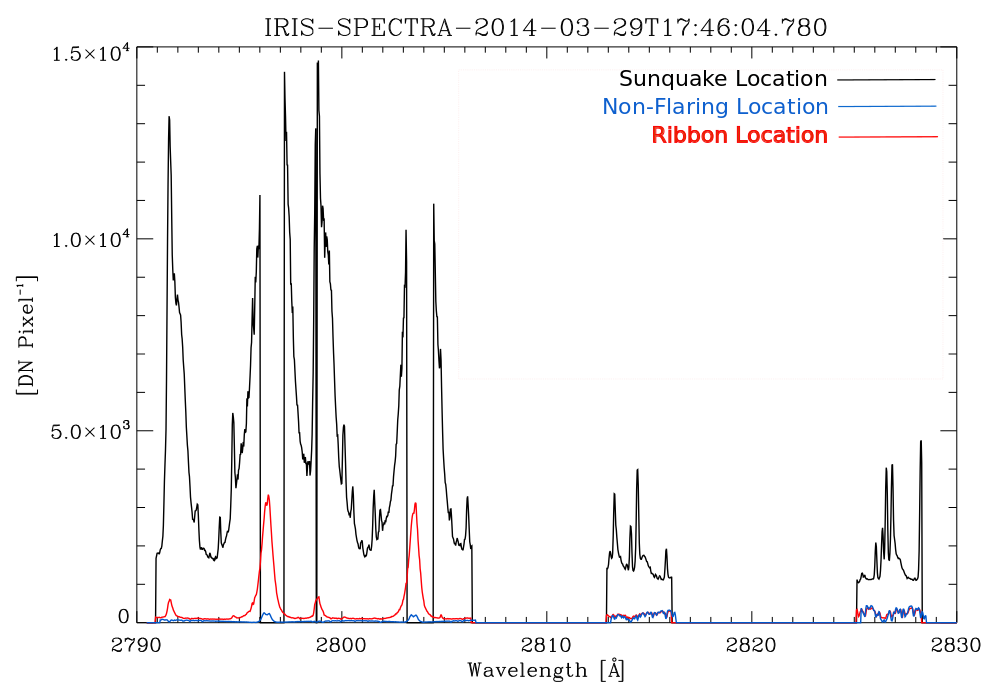
\includegraphics[width=0.58\textwidth]{spectra}
  \end{center}
  \caption{IRIS spectroscopic data ranging in wavelength 2796 - 2830Å with a smaller plot showing a zoom of the region containing the Mg II triplet lines. Black is the spectrum at the quake location (y = 435), red is the spectrum at a point along the ribbon (y = 489) and blue is the spectrum of a non-flaring region (y = 20). Square trough like features represent saturation of the CCD.}
\end{figure}
 

\subsection{First Results and Discussion}
The location of maximum acoustic power, RHESSI HXR, IRIS and SDO intensity correlate both spatially and temporally \ref{saxcontours}, showing that energy input into the upper chromosphere somehow propagates down to the photosphere. Intensity lightcurves \ref{lcseries} from SDO and IRIS seem to suggest a similar representation of the movement of energy through the chromosphere to lower altitudes, since their impulsive appearance and peak intensity occur within a minute of each 
other throughout the different regions. Intensity contrast values shown in \ref{lcseries} give an idea of how much energy is being deposited in each part of the atmosphere but energy calculations are needed. A highly impulsive Balmer continuum \ref{lcseries}, at sunquake and ribbon locations, shows that there is likely to be some radiative backwarming involved in passing energy to the photosphere. Spectroscopic data shown in \ref{spectra} show the sunquake emission to be an order of magnitude greater in amplitude than in the ribbon. The spectrum taken from a non-flaring region is around three orders of magnitude smaller than the sunquake location. Lines over the sunquake location are strongly broadened when compared to spectra elsewhere \ref{spectra}. Ribbon and sunquake spectra appear to be slightly redshifted in comparison to the non-flaring region.\\


\subsection{Future Work}
Calculate energy associated with emission captured by HMI to compare with the acoustic power of the sunquake. Calculate energy associated with emission captured by IRIS slit jaw and spectrometer in order to estimate energy deposition in the atmosphere. Calculate energy associated with Balmer emission to assess likely energy contribution of radiative backwarming. Calculate non-thermal electron power via HXR spectra to estimate the initial energy of the electron beam accelerated by the corona. A more detailed analysis of IRIS spectroscopic data to estimate velocity, density and temperature of chromospheric material. Analysis of triplet lines in the wings of Mg II h \& k will be used to determine heating of the lower chromosphere. Compare spectroscopic data taken by EIS with that of IRIS. Magnetogram: Look at HMI/SOT data to analyse the configuration of the magnetic field.\\



\subsubsection{Energy Calculations}
Due to the forethought of Lockheed Martin, the IRIS spacecraft has trustworthy pre-launch calibrations, which are time evolved to take into account degredation of the CCD.......

\begin{equation}
F(erg.s^{-1}.cm^{-2}.\AA^{-1}.sr^{-1}) = F(DN)\frac{E_{\lambda}\text{DN2PHOT_SG}}{A_{eff}\text{Pix}_{xy}\text{\lambda}t_{exp}W_{\text{slit}}}
\end{equation}

where photon energy is $E_{\lambda}=\frac{h.c}{\lambda}$, $\text{DN2PHOT_SG}$ is the number of photons per DN, $A_{eff}$ is effective area in $cm^{-2}$, $\text{Pix_{xy}}$ is spatial pixel size in radians, $\text{Pix_{\lambda}}$ is the spectral pixel size in $\AA$, $t_{exp}$ is exposure time in seconds and $W_{\text{slit}}$ is the slit width ion radians. 





\label{Bibliography}
\lhead{\emph{Bibliography}}  % Change the left side page header to "Bibliography"
%\bibliographystyle{unsrtnat}  % Use the "unsrtnat" BibTeX style for formatting the Bibliography
\bibliographystyle{plainnat}%abbrv}
%\bibliography{../../Bibliography}  % The references (bibliography) information are stored in the file named "Bibliography.bib"
\bibliography{Bibliography}
\end{document}










